\section{Related Work}

\subsection{Mazemap}

\subsection{Google Maps}
\label{Google Maps}

In March 2011, Google introduced the first indoor floorplans in their map. The intention was to increase the overview in public areas like train stations, malls and airports.
Users can upload own floorplans (valid formats include for example PNG, PDF or JPEG) to the map, with restriction to only publicly available areas.

Google Maps also offers a very popular API for their services. This allows the integration of the Google Maps Services in your own website. The usage is free for commercial use up until 28000 calls per day\footnote{According to \url{https://cloud.google.com/maps-platform/pricing/sheet/?hl=de}} and requires an API key.
The Maps JavaScript API comes with direct support for importing GeoJSON and can be customized with own content. Its designed to load maps quickly and is optimized for mobile use. Aside from that it also offers a versatile visualization library, which also includes a Heatmap Layer that helps with visualizing a heatmap (Figure 2.1.).

\begin{figure}[!hb]
	\centering
	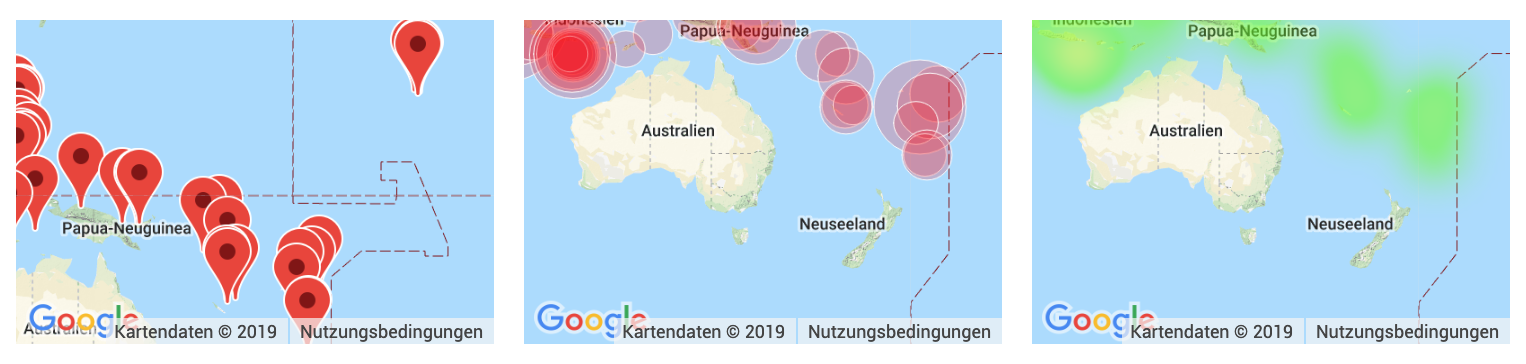
\includegraphics[width=1\linewidth]{images/GoogleMapsHeatmap}
	\caption{Example of visualization options in Google Maps}
	\label{fig:GoogleMapsHeatmap}
\end{figure}

Although this looks very promising for creating our indoor floorplan, there are quite a few problems for us.

Because the API needs an internet connection, offline development is not possible. 
Furthermore the Google Maps API would request payment after hitting the threshold of API calls mentioned above and therefore needs to be linked to an account where billing is activated. Although hitting this threshold could only happen in production, our project partner set the requirement to only use free and also open-source software and linking a billing account of our partner to use the API was not possible. 

Therefore Google Maps was not applicable to our task of creating an interactive floorplan.

\subsection{OpenLayers}
\label{OpenLayers}

OpenLayers is an open-source JavaScript library for displaying interactive maps. Out of the box it comes with various features like map rotation, direct mobile support and import of GeoJSON, TopoJSON, KML\footnote{Keyhole Markup Language} or GML\footnote{Geography Markup Language} data \footnote{\url{https://openlayers.org/}}. Unlike Google Maps, OpenLayers is a pure client-side library with no server-side dependencies. 

Because it has a lot of features already bundled together, it offers far more functionality than we need to meet the requirements of our floorplan. 

This also results in a heavyweight module. With a minified bundle size of 330.1 kB (Version 5.3.3) it takes up to 1.6 seconds to download on 3G\footnote{\url{https://bundlephobia.com/result?p=ol@5.3.3}}. Although this can be lowered for production by deleting unused modules, it takes extra effort to see which modules are really not used.

Due to the limited time we had for the implementation of the floorplan (due to it being the last feature on our roadmap) and only beginner knowledge of JavaScript, we needed something that is easy to understand and lets beginners output something useful in a short time. Because the abstraction layer of OpenLayers  is quite low, the learning curve can be pretty steap. Compared to Leaflet it takes a lot more code to get the same results.

Therefore we thought that OpenLayers doesn't fit our task.

\clearpage